\documentclass[11pt]{article}

\usepackage[top=0.5in, bottom=0.5in, left=0.5in, right=0.5in]{geometry}
\usepackage{authblk}
\usepackage{hyperref}
\usepackage[utf8]{inputenc}
\usepackage{amsmath}
\usepackage{amsfonts}
\usepackage{amssymb}
\usepackage{siunitx}
\usepackage{graphicx}
\usepackage{subcaption}
\usepackage{float}
\usepackage[nottoc,numbib]{tocbibind}
\usepackage{biblatex}

\bibliography{references.bib}

\newcommand{\email}[1]{\texttt{\href{mailto:#1}{#1}}}

\title{CMSC 478 Project Final Report}
\author{Robert Rose}

\makeatletter
\let\inserttitle\@title
\let\insertauthor\@author
\makeatother

\begin{document}

\begin{center}
  \LARGE{\inserttitle}

  \Large{\insertauthor}
\end{center}

\section{Introduction}

My project is based off of a currently running Kaggle competition to predict the winning placement of a
given player out of several hundred thousand games of the video game Player Unknown's Battle Grounds 
(PUBG). As a result the competition information and data can be found on  the Kaggle website for the 
competition.\cite{competition} Additionally, the Python notebook with my work can be found pre-rendered 
as a Kaggle Kernel, which is what I recommend using since it takes quite some time to run all the way 
through.\cite{clustering} The video game PUBG is first person shooter that pits up to 100 players against
each other on an extremely large map on teams of up to four people. The premise of my project was whether
unsupervised learning techniques such as PCA and clustering could be used to generate features that could
provide valuable information to supervised learning techniques, like most of the ones we learned in class.\\

The results were not terribly promising, at least for this dataset. Compared to a baseline Kaggle kernel 
using boosting, a Kernel trained using the unsupervised learning features performed roughly twice as
bad.\cite{baseline-lgbm} My final boosting validation score was $0.059552$, over twice the final validation
score of the baseline kernel, and not a terribly good improvement over the simple linear regression model
I used in the milestone. Additionally, one of the sample linear regression features from the kernel I got
the experiments idea from outperformed the boosting model, so it's safe to assume that the unsupervised
learning features made the model worse, not better.\cite{feature-engineering}\\

The current result puts me in the top 52\% of submissions for this competition, which is certainly better 
than a lot of people, but considering there are publicly available Kernels that outperform me, it could be
a lot better. However, the primary objective of my project was not so much to the rank as high as possible 
as it was to explore whether or not unsupervised learning techniques could generate useful features.

\section{Techniques}

Unsupervised learning is the subset of machine learning that does not require labeled data in order
to gain information about the dataset. Instead of using a training set with labels to learn about the data,
unsupervised learning works solely off of the relationships and distribution of the training data. I used
two unsupervised learning techniques for this project: clustering and principal component analysis (PCA).
Although PCA is nominally an unsupervised learning technique, I used it for dimensionality reduction prior
to using $K$-means clustering on the data to generate features.\\

Using PCA I was able to reduce the data down into two dimensions, as seen in the two graphs below. Using
only two PCA components, I was able to explain 74.9\% of the variance in the data. Using three components,
I was able to explain nearly 95\% of the variance, but I chose to stick with only two as it made the centroids 
features more meaningful. 

\begin{figure}[h]
\caption{Data After PCA}
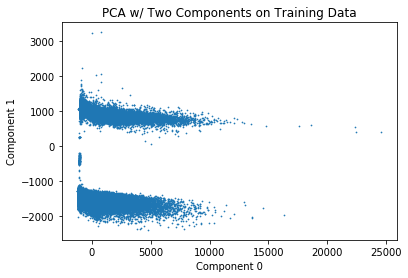
\includegraphics[width=0.6\textwidth]{imgs/train_pca.png}
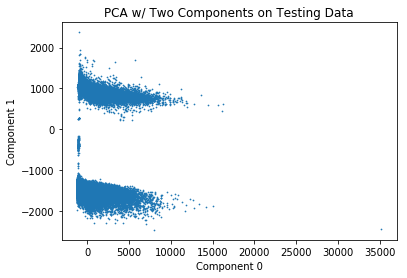
\includegraphics[width=0.6\textwidth]{imgs/test_pca.png}
\centering
\end{figure}

The two features I attempted to generate using clustering were then centroid distances and which cluster a
point was in. Centroids were calculated by simply taking the euclidean distance between each point's two 
PCA components and the center of each of the clusters. The cluster membership was simply a one-hot encoded
variable for each of the clusters, $1$ if a point was in that cluster and $0$ otherwise.\\

Early on I was hoping that I would be able to use a clustering method that would converge on the north and
south clusters seen in Figure 1. Unfortunately I was unable to find a clustering algorithm that
would converge on those two clusters. $K$-means with 2 clusters converged on the "head" and "tail" of the two
clusters and I was unable to find DBSCAN parameters that satisfactorily clustered the data. So instead I used
$K$-means with three, four and five clusters to generate centroids and cluster memberships.\\

I chose not to use any cross-validation techniques such as $K$-fold for my project as I felt they would be
unnecessary since the dataset was sufficiently large enough to generate a training and validation set on its
own. I did find that for some of the match types, there were only a few hundred entries in the training set.
However, these were mostly for custom match modes that only played a few games, and since I was splitting on
matchId, they would be unlikely to make it into both the validation and training set. For the validation set
which ended up without them, I simply set those columns to zero so it would work correctly in LightGBM.
For assessing model accuracy I used the metric for the competition that would be used to score submissions, 
mean absolute error.\\

I used two types of models we talked about in class in my project: boosting, via the LightGBM library, for
the final prediction and linear regression, via Sci-kit Learn, for testing features in the project
milestone.\cite{ke2017lightgbm}\cite{scikit-learn} Linear regression was useful in the feature selection,
and in the milestone I called the results from it "fairly promising". In hindsight however, I probably should
have been more cautious about continuing down this path of the project considering how little of an improvement
the unsupervised learning methods had over the original dataset. While I attributed their poor performance to 
linear regression being unable to properly handle their input, it's probable they were just poor predictors
and the improvement they got over the original dataset was by chance.

\begin{table}[h]
 \centering
 \caption{Cluster and Centroid Simple Model Results}
 \begin{tabular}{||c c c c||} 
 \hline
 Index & Name & Score & Execution Time \\ [0.5ex] 
 \hline\hline
 4 & kmeans\_4\_centroids & 0.089267 &	47.68s \\ 
 \hline
 5 & kmeans\_5\_clusters & 0.089349 & 47.73s \\
 \hline
 1 & kmeans\_3\_clusters & 0.089359 &	46.66s \\
 \hline
 6 & kmeans\_5\_centroids & 0.089408 &	48.28s \\
 \hline
 3 & kmeans\_4\_clusters & 0.089562 & 48.72s \\
 \hline
 2 & kmeans\_3\_centroids & 0.089677 & 47.29s \\
 \hline
 0 & original &	0.092813 & 28.97s \\ 
 \hline
\end{tabular}
\end{table}

\section{Reflection}

Overall, this project was not as successful or meaningful as I had hoped. I was hoping using unsupervised learning
techniques to generate features would be a novel approach that would yield interesting results that could be applied
to future projects I work on. Unfortunately, that doesn't look like it's the case. There's arguably improvements that
could be made in model hyperparameter tuning, but due to the poor results I got from using a baseline Kernel's parameters,
I highly doubt better hyperparameters could make up for the poor performance, especially when its current performance is
comparable to team-based aggregate features with linear regression.\cite{feature-engineering}\\

While I could likely include some of those parameters in my model for a performance gain, that would defeat the purpose
of my project exploring the use of unsupervised learning techniques for feature engineering. Overall I think I learned a lot
however, in the future I likely won't spend time attempting things like this and will just stick with simple ensembling and
neural nets. At the very least, I will stick with what other peers are showing positive results with, at least in Kaggle
competitions.

\printbibliography

\end{document}